\section{Abu Dhabi Grand Prix}

\subsection{Circuit Analysis}

\textbf{Circuit Name:} Yas Marina Circuit (Abu Dhabi, United Arab Emirates) \\
\textbf{Length:} 5.281 km - \textbf{Laps:} 58 - \textbf{Total Distance:} 306.183 km

\begin{figure}[H]
    \centering
    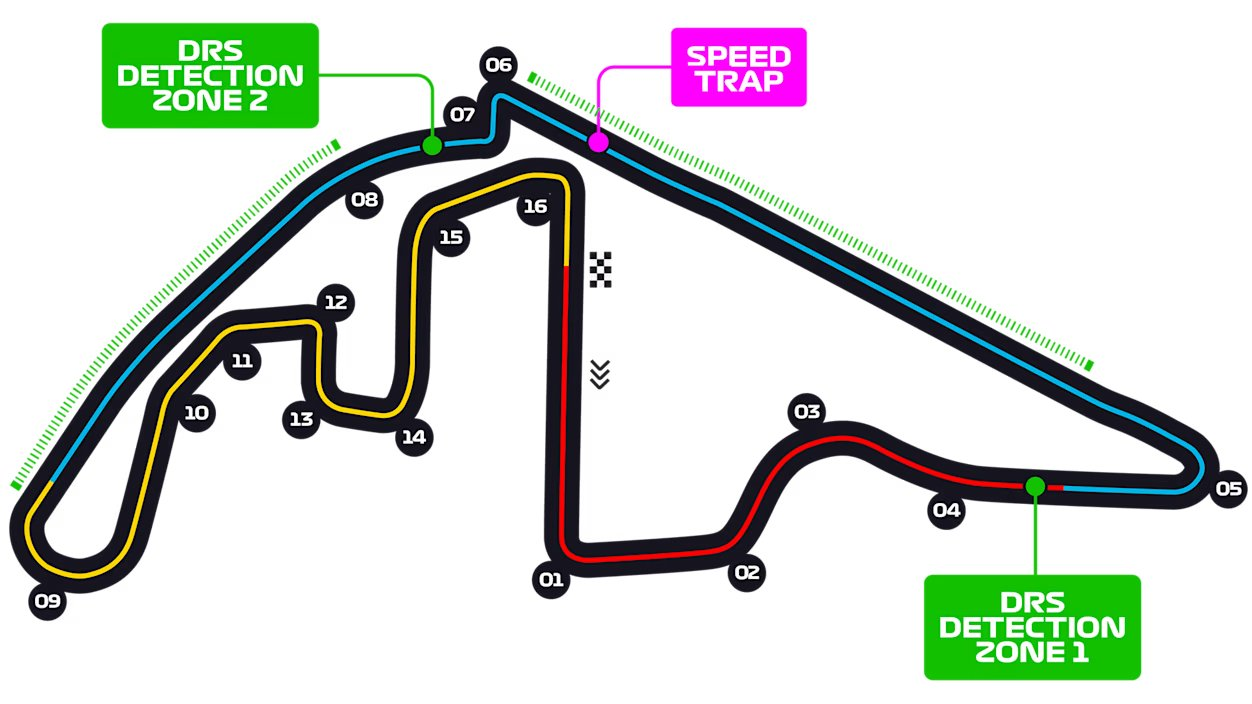
\includegraphics[width=0.75\linewidth]{images/24.Abu_Dhabi_Circuit.jpg}
\end{figure}

\begin{itemize}
    \item \textbf{Lap Record} : 1:23.445 (2023, Max Verstappen – Red Bull). 

    \item \textbf{Number of Corners \& Key Features} : 16 turns (9 right, 7 left). \\
    Features two long straights with heavy braking (Turns 6 and 9), plus a technical third sector. 
    The track layout was revised in 2021 to improve overtaking.

    \item \textbf{Braking Zones \& Traction} : Turn 6 and Turn 9 are prime overtaking zones, requiring strong braking stability. \\
    Sector 3 demands traction and downforce for slow corners leading onto the main straight.

    \item \textbf{DRS \& Overtaking} : Two DRS zones (post-Turn 5 chicane and between Turns 8 and 9). \\
    Overtaking remains challenging but possible with strong exit speed.

    \item \textbf{Tyre Degradation \& Strategy} : Low to medium degradation thanks to smooth asphalt. \\
    One-stop strategies common, but safety cars can shuffle tactics.

    \item \textbf{Weather \& Environment} : Twilight-to-night race under floodlights. \\
    Track temperature drops during the race, aiding tyre management but complicating balance.
\end{itemize}

\textbf{Strategic Summary :} Yas Marina requires aerodynamic efficiency, braking stability, and tyre consistency. The shifting track conditions add complexity to race strategy.

\subsection{Race Analysis}

\textbf{Date:} 8 December 2024 — 17:00 local time 

\begin{itemize}
    \item \textbf{Qualifying Summary} : \textbf{Pole Position:} Lando Norris (McLaren) – 1:22.595 (new track record). \\
    Grid: Piastri 2nd, Sainz 3rd, Verstappen 4th. \\
    Leclerc penalised for power unit change (P19 start). \\
    Hülkenberg dropped from P4 to P7 for pitlane infraction.

    \item \textbf{Race Summary} : \textbf{Winner:} Lando Norris (McLaren) — sealing McLaren’s Constructors’ title. \\
    \textbf{Podium:} 1. Norris - 2. Sainz - 3. Leclerc. \\
    \textbf{Notable incidents:} Verstappen collided with Piastri at Turn 1 (10s penalty, finished P6). Piastri penalised for clash with Colapinto (P10). \\
    Pérez retired lap 1. Bottas and Colapinto also DNFs. Hamilton (hard tyre start) charged from P16 to P4 in his Mercedes farewell.

    \item \textbf{Strategies} : \\
    - McLaren: Norris flawless, Piastri compromised by contact + penalty. \\
    - Ferrari: Sainz P2 (last race with Ferrari), Leclerc P3 from P19 after stunning comeback. \\
    - Mercedes: Hamilton emotional P4 in last race with Mercedes, Russell P5. \\
    - Red Bull: Verstappen salvaged P6 despite penalty, Pérez retired immediately. \\
    - Alpine: Gasly P7 secured Alpine P6 in Constructors’. \\
    - Haas: Hülkenberg P8 solid, Magnussen P16 but fastest lap. \\
    - Alpine rookie debut: Jack Doohan P15, steady first race.

    \item \textbf{Performance Trends} : \textbf{McLaren} dominant with Norris’ pole-to-win.\\
    \textbf{Ferrari} maximised points with both cars on podium. \\
    \textbf{Mercedes} ended strongly with Hamilton’s charge. \\
    \textbf{Red Bull} struggled: Verstappen penalised, Pérez DNF. \\
    \textbf{Alpine} defended crucial P6 in Constructors’.\\
    \textbf{Haas} again competitive with Hülkenberg and fastest lap for Magnussen.

    \item \textbf{Championship Impact} : \\
    \textbf{Drivers:} Verstappen 437 pts (Champion), Norris 374, Leclerc 356. \\
    \textbf{Constructors:} McLaren 666 (Champion), Ferrari 652, Red Bull 589, Mercedes 468. \\
    McLaren clinched first Constructors’ title since 1998.
\end{itemize}

\textbf{Key Takeaway :} Lando Norris dominated Abu Dhabi to crown McLaren Constructors’ Champions for the first time in 26 years. Ferrari’s double podium fell just short, Verstappen ended season on a muted note, while Hamilton delivered a farewell masterclass for Mercedes. Alpine clinched P6 in the standings, Zhou secured Kick Sauber’s first points season since 2022. The 2024 finale sealed a historic McLaren resurgence.

\subsection{Link \& Takeaway}

\begin{itemize}
    \item McLaren sealed their first Constructors’ title since 1998 with a flawless weekend led by Norris. 
    \item Ferrari fought valiantly, but Leclerc’s comeback and Sainz’s podium couldn’t overturn the deficit. 
    \item Verstappen penalised and Pérez retired: Red Bull ended season below expectations. 
    \item Hamilton signed off his Mercedes career with a remarkable recovery drive to P4. 
    \item Alpine’s Gasly defended hard to secure P6 in Constructors’, Haas showed flashes with Hülkenberg and Magnussen. 
    \item Abu Dhabi 2024 will be remembered as the race where McLaren returned to the summit of Formula 1.
\end{itemize}
